\section{Design Summary}

The design of this device encompasses three main sections; the DAW, the Autofill Feature,
and the Keyboard interface. The integration of these three sections will create the final
product. The DAW will manage the MIDI files and display any changes that occur from the
keyboard or Autofill feature. The Autofill feature will take the current MIDI file from
the daw and generate suggestions for imporovements and future notes to be added to the
MIDI file. The Keyboard will be the method of imputting new notes or chords to the DAW and
subsequently the MIDI files. The combination of all three of these task is what our design
seeks to accomplish.

\begin{figure}[h!]
  \centering
  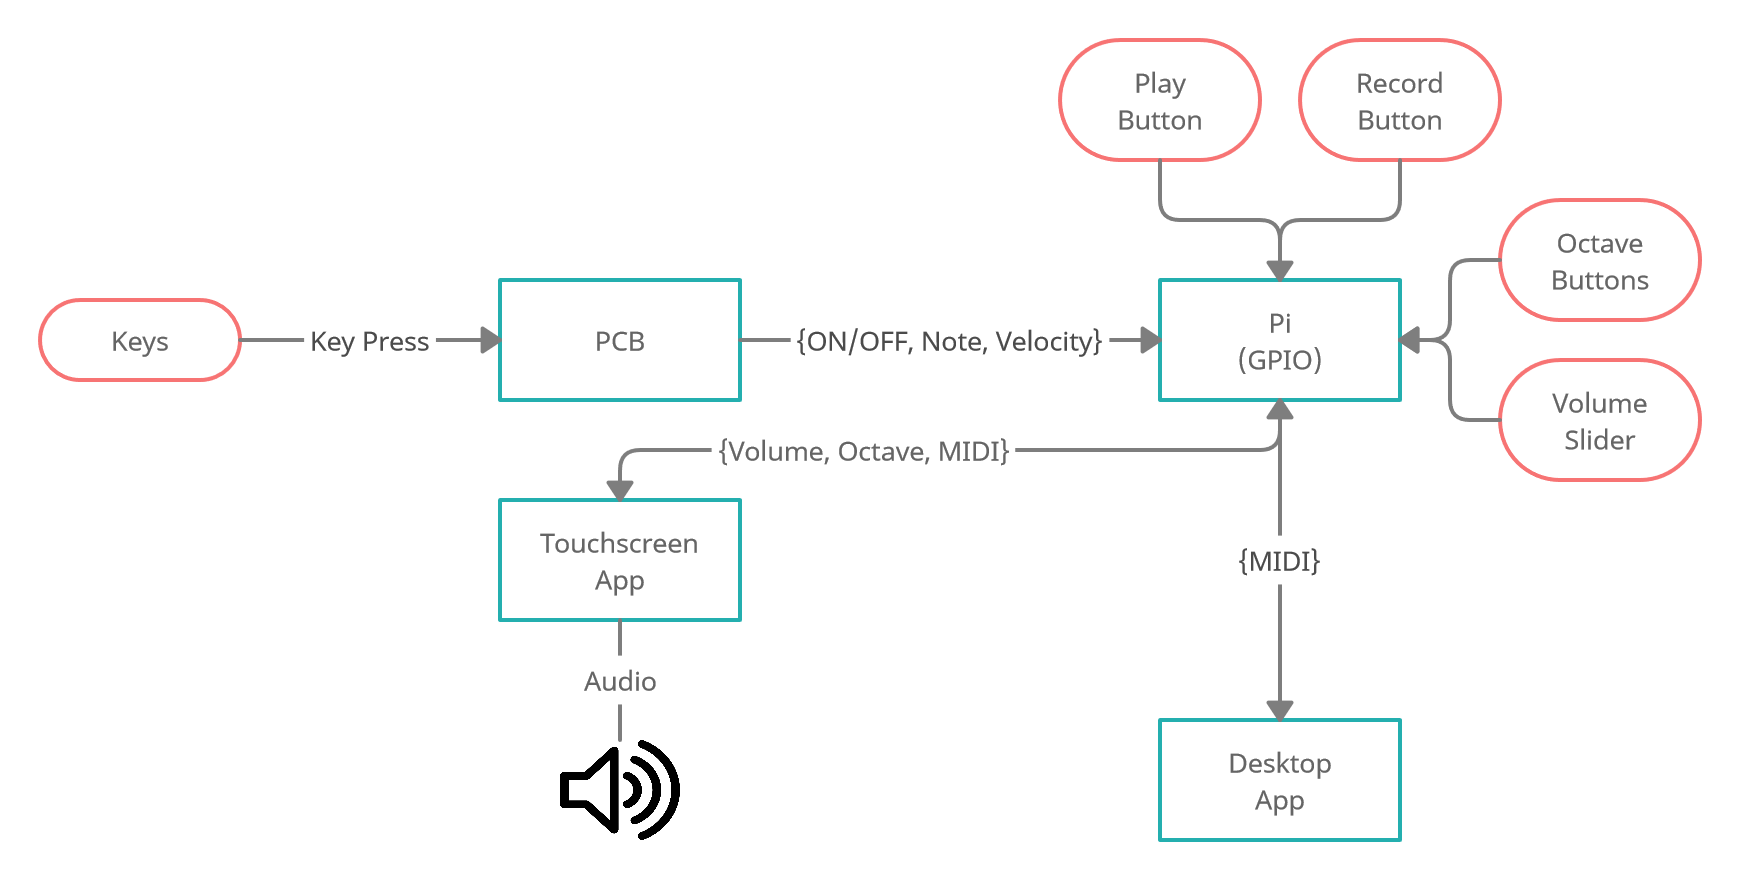
\includegraphics[width=\linewidth]{image/BlockDiagram.png}
  \caption{The flow of information and control.}
  \label{fig:block_diagram}
\end{figure}

\newpage
\subsection{Keyboard}

The keyboard will act as the physical interface that users interact with when inputting to
the DAW. This section encompasses the metronome, keys, volume control, record, and play
features. Each input affects the resulting Audio Playback and subsequently gives that data
to the DAW, which will act as the main controller of the entire system.
\autoref{fig:keyboard_diagram} encompasses this idea in a compressed and streamlined
graphic.

\begin{figure}[h!]
  \centering
  \includegraphics[width=\linewidth]{image/Keyboard.png}
  \caption{The overall structure of the project.}
  \label{fig:keyboard_diagram}
\end{figure}

\newpage
\subsection{DAW}

The DAW will act as the central location where MIDI files will be created and stored. It
will take inputs from the Keyboard and give complete MIDI files to the Autofill AI. It
will also allow the user to adjust and place notes that they believe require adjustment.
The DAW feature will allow for a centralized and streamlined processing of inputs and
outputs as well as an interface for the user to interact with the MIDI controller.

\begin{figure}[h!]
  \centering
  \includegraphics[width=\linewidth]{image/DAW.png}
  \caption{Structure of the MIDI editing component.}
  \label{fig:daw_diagram}
\end{figure}

\newpage
\subsection{Autofill Feature}

The autofill feature is the main focus of this project as it is the central idea of our
initial design meeting. The Autofill feature will extract the MIDI file generated by the
DAW and create a number of subsequent files to help the user compose melodies of
symphonies representative of the selected genre. This will be accomplished using a trained
AI that is capable of further improvements via third-party connections and processing.

\begin{figure}[h!]
  \centering
  \includegraphics[width=\linewidth]{image/Autofill.png}
  \caption{Structure of the melody autofill component.}
  \label{fig:autofill_diagram}
\end{figure}
\clearpage

\subsection{MIDI Circuit Board}

Printed circuit boards are the cornerstone to every electronics related project.
The same can be said for this MIDI keyboard with Autofill features. The first
step in creating this essential component was to determine the exact distances
and locations of each Key. Our product utilized a 2.5 octave design and
therefore needed to be exact in measurement lest minor mistakes cascade into
costly errors. I and a classmate convened and determined the optimal distance
between each keys for an octave were as followed, measured in mm. These
measurements were determined taking in mind the size of an average MIDI keyboard
as well as their distance in between each key and group of keys.

\begin{figure}[h!]
  \centering
  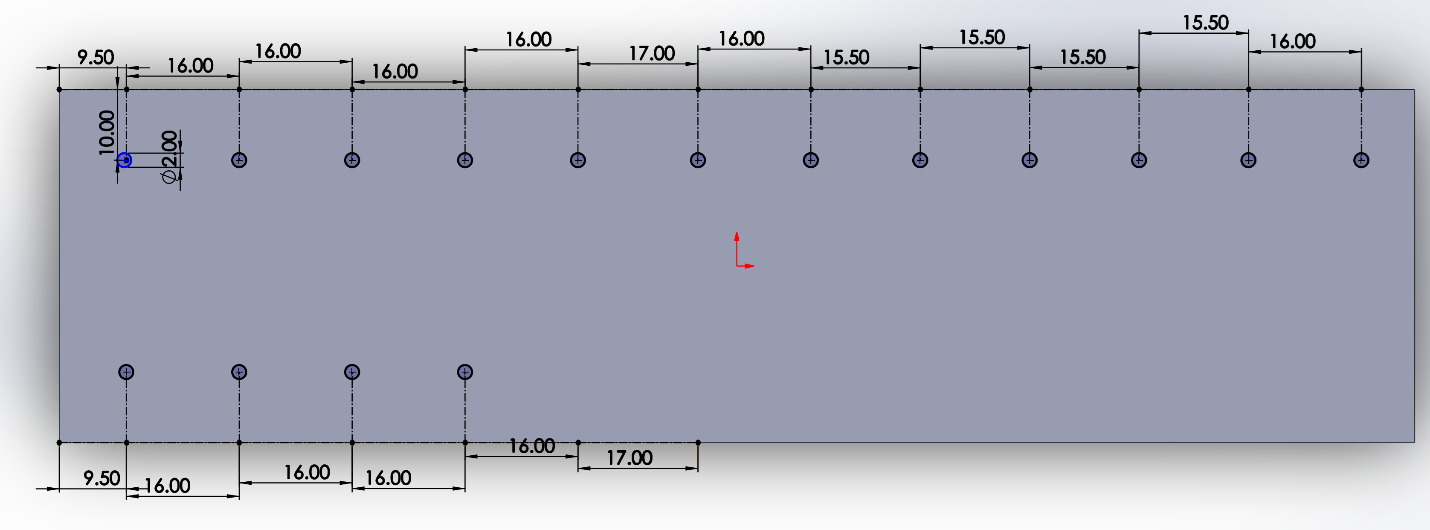
\includegraphics[width=\linewidth]{image/pcbdesign.png}
  \caption{Keyboard measurements one octave.}
  \label{fig:pcb_design_diagram}
\end{figure}

This design can be easily tessellated horizontally given that you leave exactly
17mm of space in between the latest end key and the new first key. It is also
recommended that if you are to use an incomplete octave that you either truncate
the design at the 17mm distance or add a select few keys approximately 16.50mm
away from the designed board and from each other. Failure to do say may lead to
complication when implementing, creating, or printing a housing for the circuit.
The initial design was reliant on a series of pressure sensitive buttons,
reminiscent of the controllers of old as well as a common design for many other
electronics, such as scales, touchscreens, some computer keyboards, and water
pumps. However, the price of such components far outweighed the projected
benefit of being able to know the precise pressure a user applies to a given
key. What’s more, such large designs were ineffective and wasteful for our
close-knit keyboard requirements. The smallest available we could find was at
least 13mm across, uncomfortably close for our purposes.

\begin{figure}[h!]
  \centering
  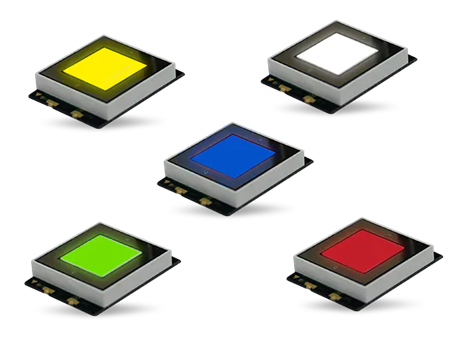
\includegraphics[width=\linewidth]{image/pressuresensitivebuttons.png}
  \caption{Pressure sensitive buttons.}
\end{figure}


Thusly, a different more compact option was selected, and a new design drawn up, utilizing
two simple buttons and their subsequent time delay to calculate the resultant velocity of
a given keypress. This is the specific calculation utilized when attempting to find that
velocity.

\begin{equation*}
  y = e^{-(\frac{\Delta t}{50})} * 97 + 30
\end{equation*}

This calculation ensured that we could preserve the ability for the MIDI keyboard to
differentiate between a soft keypress and a hard keypress, a staple when it comes to
creating and playing melodies on instruments in general. This is the graph of that
equation to visualize the potential range of values for the velocity calculation.

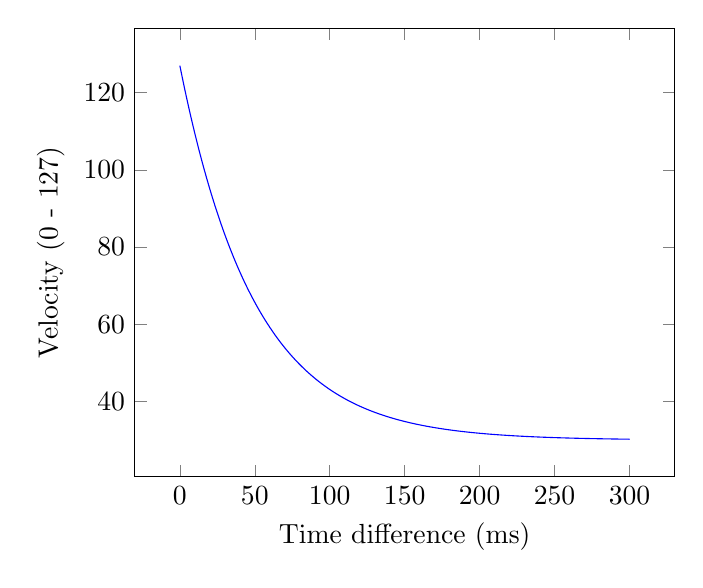
\begin{tikzpicture}
  \begin{axis}[
      domain=0:300,
      samples=101,
      smooth,
      no markers,
      xlabel = Time difference (ms),
      ylabel = Velocity (0 - 127)
    ]
    \addplot {exp(-x/50) * 97 + 30};
  \end{axis}
\end{tikzpicture}

To ensure the circuit had as accurate a measurement of time as possible, we selected a
series of soft-touch keys that use rubber pads instead of hard metals and plastic to hold
and press the contact. This allows for precise time delay measurements during the critical
keystroke.

\begin{figure}[h!]
  \centering
  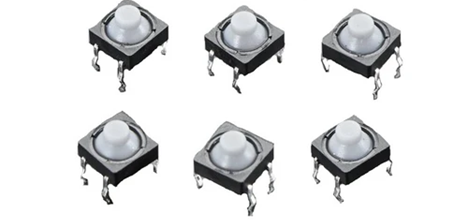
\includegraphics[width=\linewidth]{image/softtouchswitches.png}
  \caption{Soft touch switches.}
\end{figure}


Utilizing these switches as well as a resistor to reduce noise in the signal will allow us
to have a range of potential velocities be measured with reference to how rapidly the
users taps on each individual key. A standard 9.2mm resistor is all that is necessary. No
special connection nor unusual values necessary for this component of the circuit board.
For our case, a normal 1k Ohm resistor was used once the circuit was built and arrived.
Power on the left side and a ground beneath the resistor allows the switch to act as a low
noise signal to the component in front of it, allowing us to measure if that specific key
is pressed or not.

\begin{figure}[h!]
  \centering
  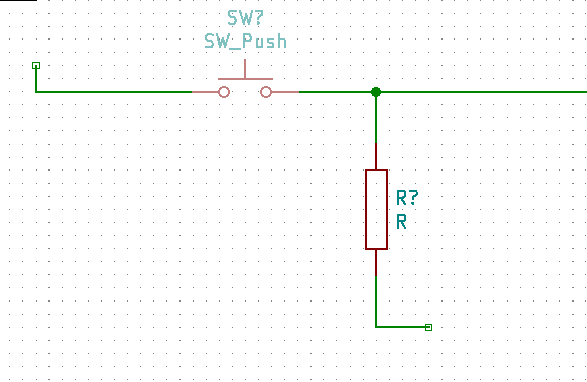
\includegraphics[width=\linewidth]{image/buttonschematic.png}
  \caption{Button schematic.}
\end{figure}

This is all well and good, but in order to create a functioning circuit we must also
determine the best means of extracting and calculating the correct signals. With our
projected design, utilizing two buttons to calculate velocity, the total number of
possible measurements balloons from a mere 29 to 58 points of interest in total. This
large number is unruly and cumbersome in the best of times and with a project such as
this, there does not exist a cheap and readily available microcontroller capable to
reading to many inputs at once. As a result, the circuit itself must include a means of
reducing the number of input and output requirements from potentially 60 total ports to
something far more manageable. Fortunately, such a design exists. They are called
multiplexers and they allow for a large number of inputs to be turned into a much smaller
number based on how many Serial inputs are used. These inputs are marks as Sn where the
smaller the n indicates the smaller the value.

\begin{figure}[h!]
  \centering
  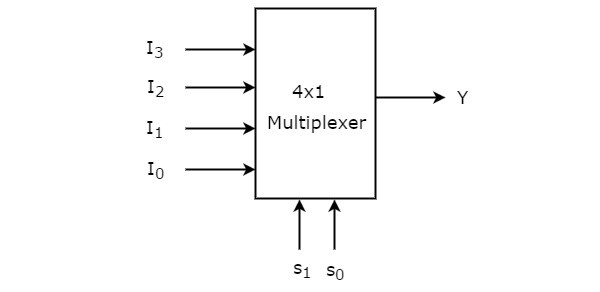
\includegraphics[width=\linewidth]{image/multiplexorconcept.jpg}
  \caption{Multiplexor concept.}
\end{figure}

Utilized in a wide variety of visual or display electronics, multiplexer and the speed of
modern computers allows for a near seamless signaling of a large number of outputs. The
same can also be done for measured inputs, allowing us to reduce the number of outputs
from our 58 keys down to just over a handful. For the purposes of our product, we are able
to reduce the staggering 60 ports in total to just a mere 9; 2 for the power and ground, 5
for the serial input, and 2 for the two resultant outputs. We could attempt to reduce the
outputs once more by adding an additional serial input, but that would be a moot point as
the number of ports would remain unchanged and merely add unnecessary complexity to our
circuit. In any regard, this is what such a multiplexer circuit would look like, at least
for a small portion of it.

\begin{figure}[h!]
  \centering
  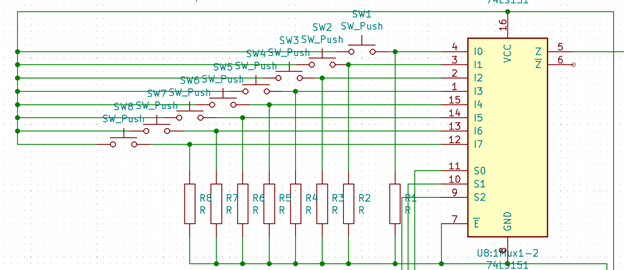
\includegraphics[width=\linewidth]{image/signaledmultiplexor.png}
  \caption{Signaled multiplexor.}
\end{figure}


Given the 29 required keys and the 58 total buttons inputted, the output would need to
propagate through its own multiplexer before emerging as the desired output for a given
serial input S. However, this multiplexer would need to be of a different design to ensure
that the input of one region did not overshadow or hide the other. This is the
demonstration and implementation of that thought.

\begin{figure}[h!]
  \centering
  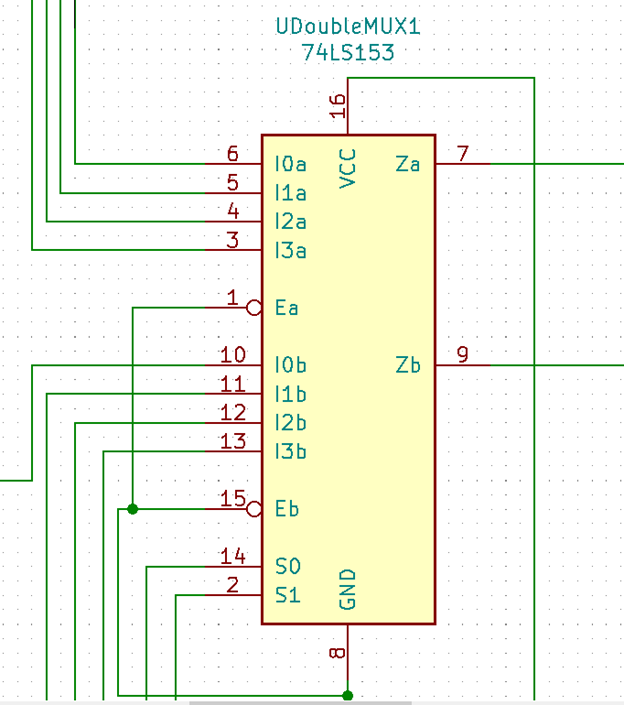
\includegraphics[width=\linewidth]{image/doublefourtoonemultiplexor.png}
  \caption{Double 4x1 multiplexor schematic.}
\end{figure}

Naturally, a single set of chips does not adequately demonstrate nor show the inner
workings of a circuit board as complex as this. Thusly, here is the full circuit being
utilized when dealing with our MIDI keyboard.

\begin{figure}[h!]
  \centering
  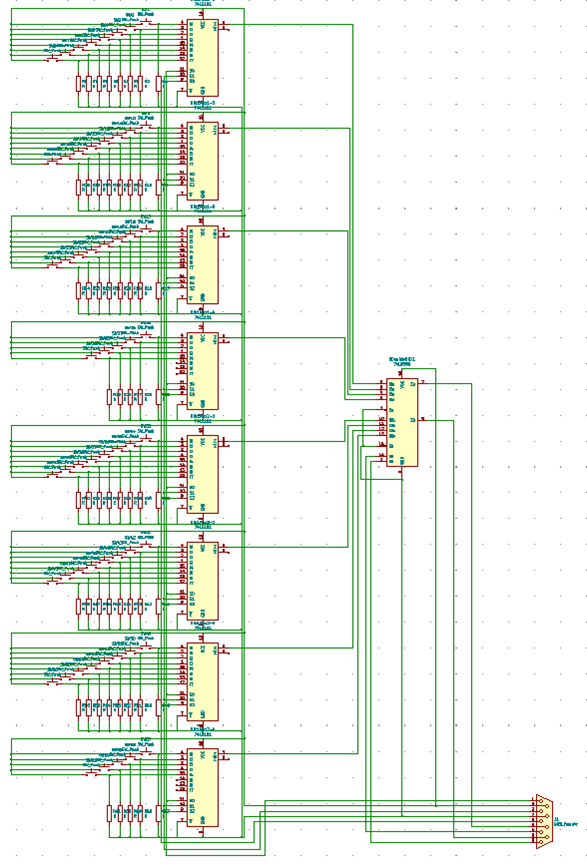
\includegraphics[width=0.5 \linewidth]{image/pcbschematic.png}
  \caption{Full PCB schematic.}
\end{figure}

Now that we have the logic design completed, we just have to design the physical circuit
and program a protocol for calculating velocity. Fortunately, now that the wires are
decided upon that matter is relatively easy to accomplish.


\begin{figure}[h!]
  \centering
  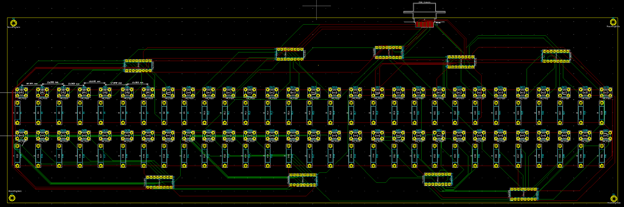
\includegraphics[width=\linewidth]{image/pcbdiagram.png}
  \caption{PCB diagram.}
\end{figure}


The physical board design is a combination of the initial key spacing as well as the
schematic design discussed earlier. The chips are place near enough to each group of
buttons while also being far enough away so as to accommodate for a wide variety of
possible wiring configurations. The power and ground ports are connected to all the
necessary components and the components are connected to the necessary locations on each
other. It is possible that a more efficient design for the board is possible. However, for
the proof of concept the board needed only to be functional and not perfect in its
efficiency. Once the final board design was presented and approved, it was sent to be
manufactured.

\begin{figure}[h!]
  \centering
  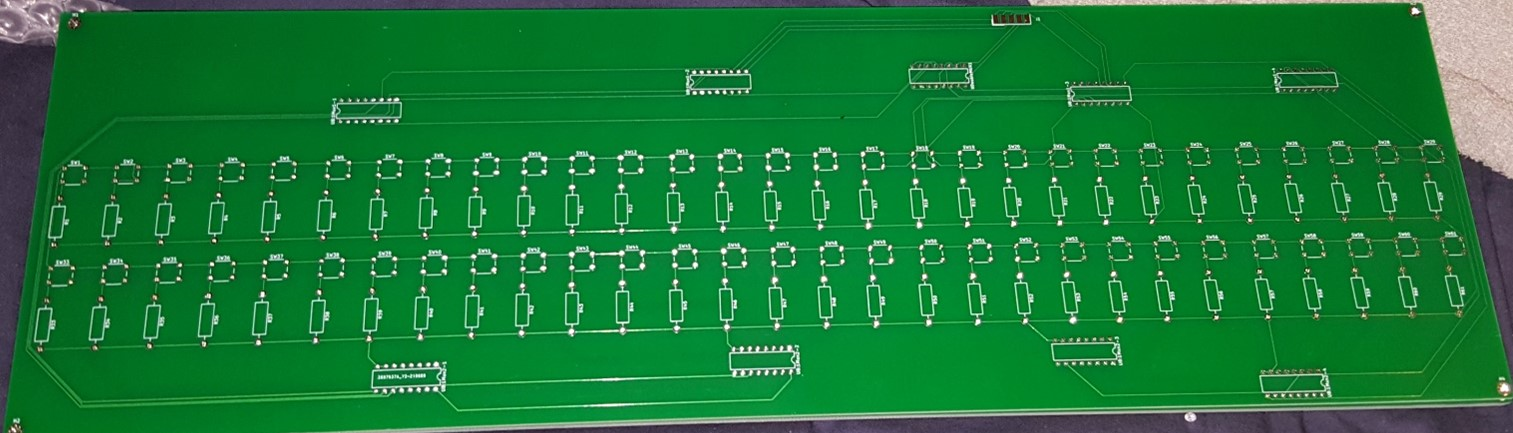
\includegraphics[width=\linewidth]{image/printedpcb.jpg}
  \caption{Blank PCB.}
\end{figure}

The components then needed to be placed and soldered to the board before integrated
testing could begin. Fortunately, the university have a lab for just such a requirement.
As a word of advice, do not focus too intently on soldering on part for too long. The heat
from the iron is easily able to transfer into the subsequent component and increase or
even cause damage to the component being attached. In total it took about 4 hours, but the
physical circuit could finally begin testing.

\begin{figure}[h!]
  \centering
  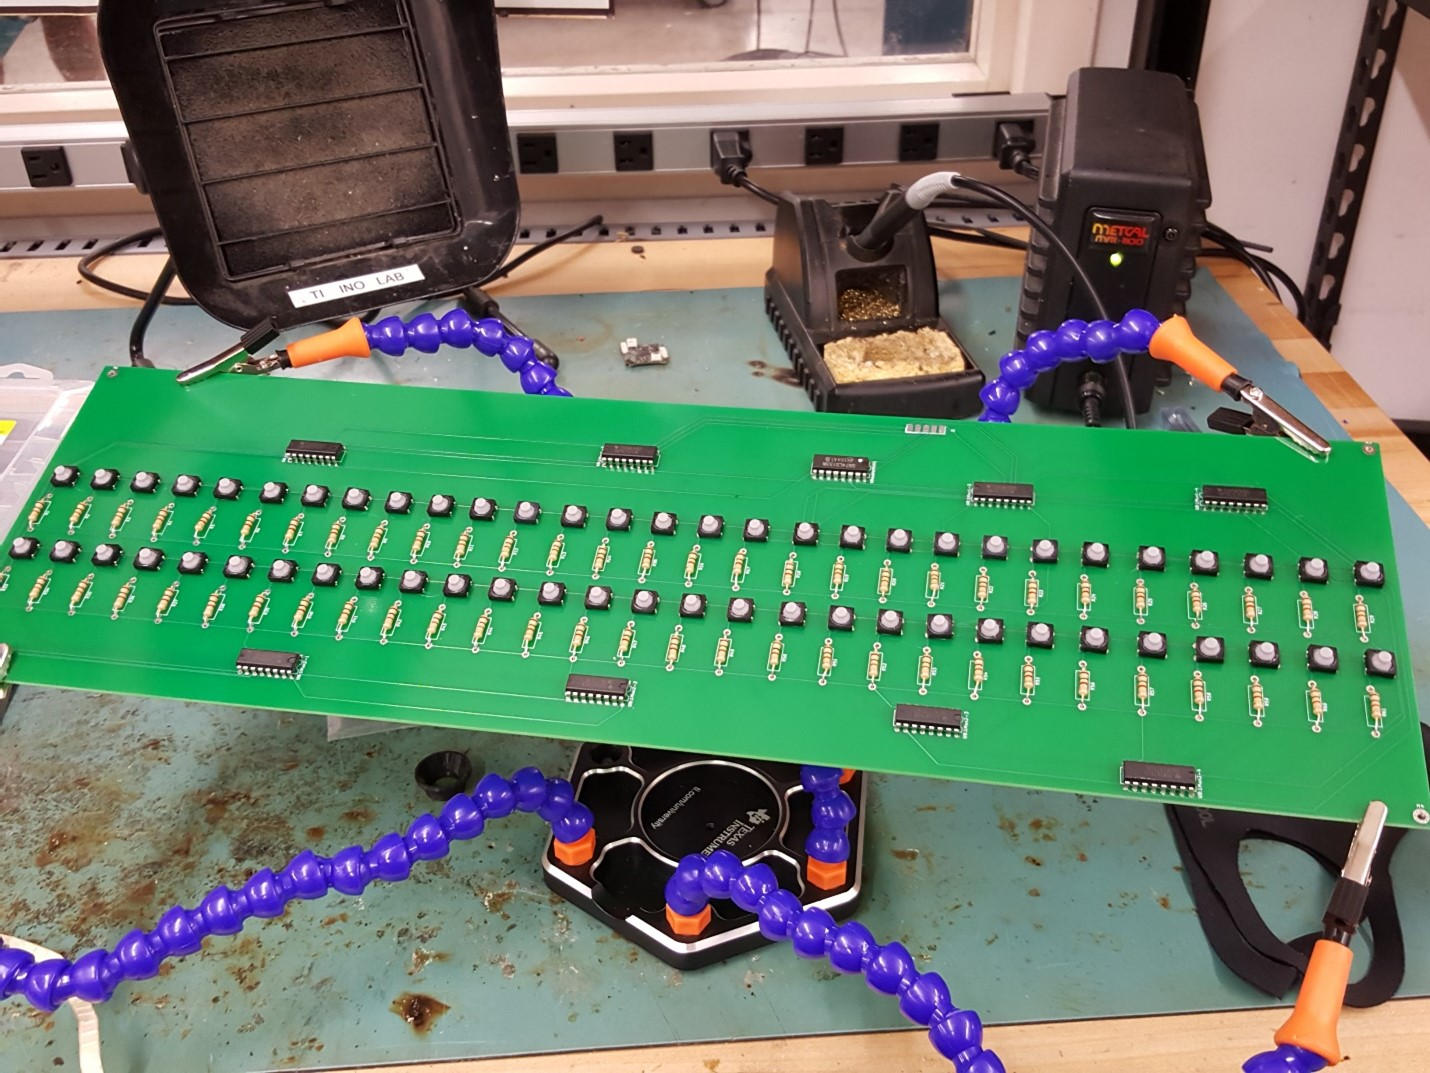
\includegraphics[width=\linewidth]{image/completedpcb.jpg}
  \caption{The completed PCB.}
\end{figure}

\begin{figure}[h!]
  \centering
  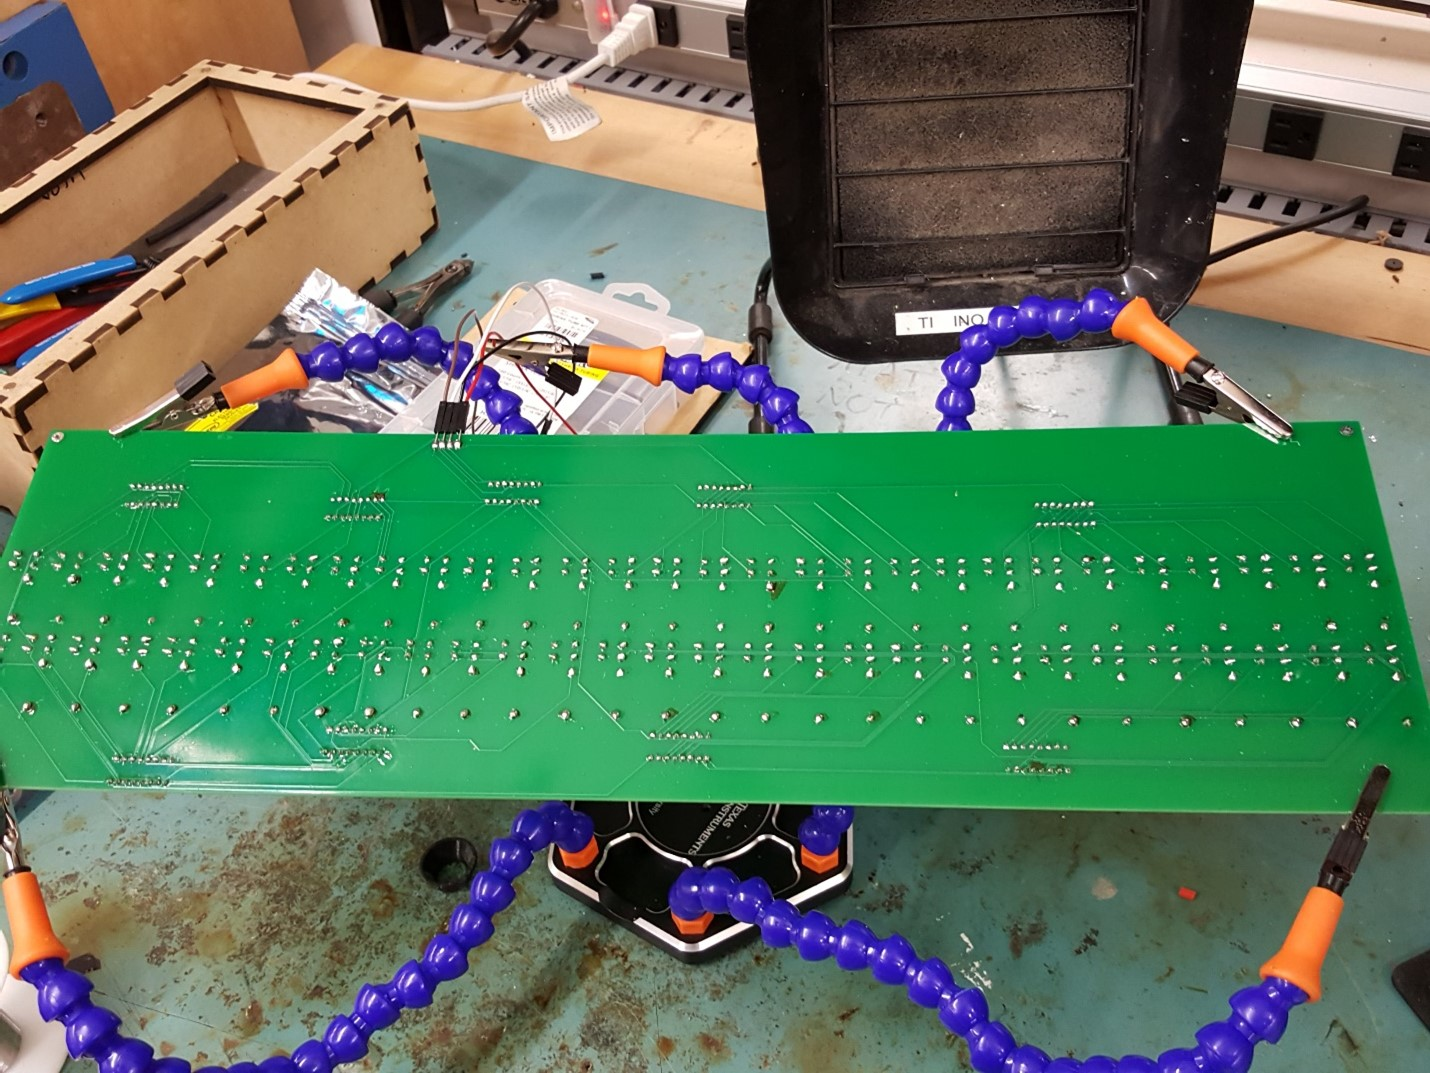
\includegraphics[width=\linewidth]{image/bottomofpcb.jpg}
  \caption{The bottom side of the completed PCB.}
\end{figure}

Naturally, we also had to connect a means of communicating with the board as the transfer
port shown in the pcb schematic would not be adequate for our needs. So, it was decided to
solder wires directly to the surface mounts, coded by color to ensure that no mistakes
could be made in connecting the board to our Arduino circuit.

\begin{figure}[h!]
  \centering
  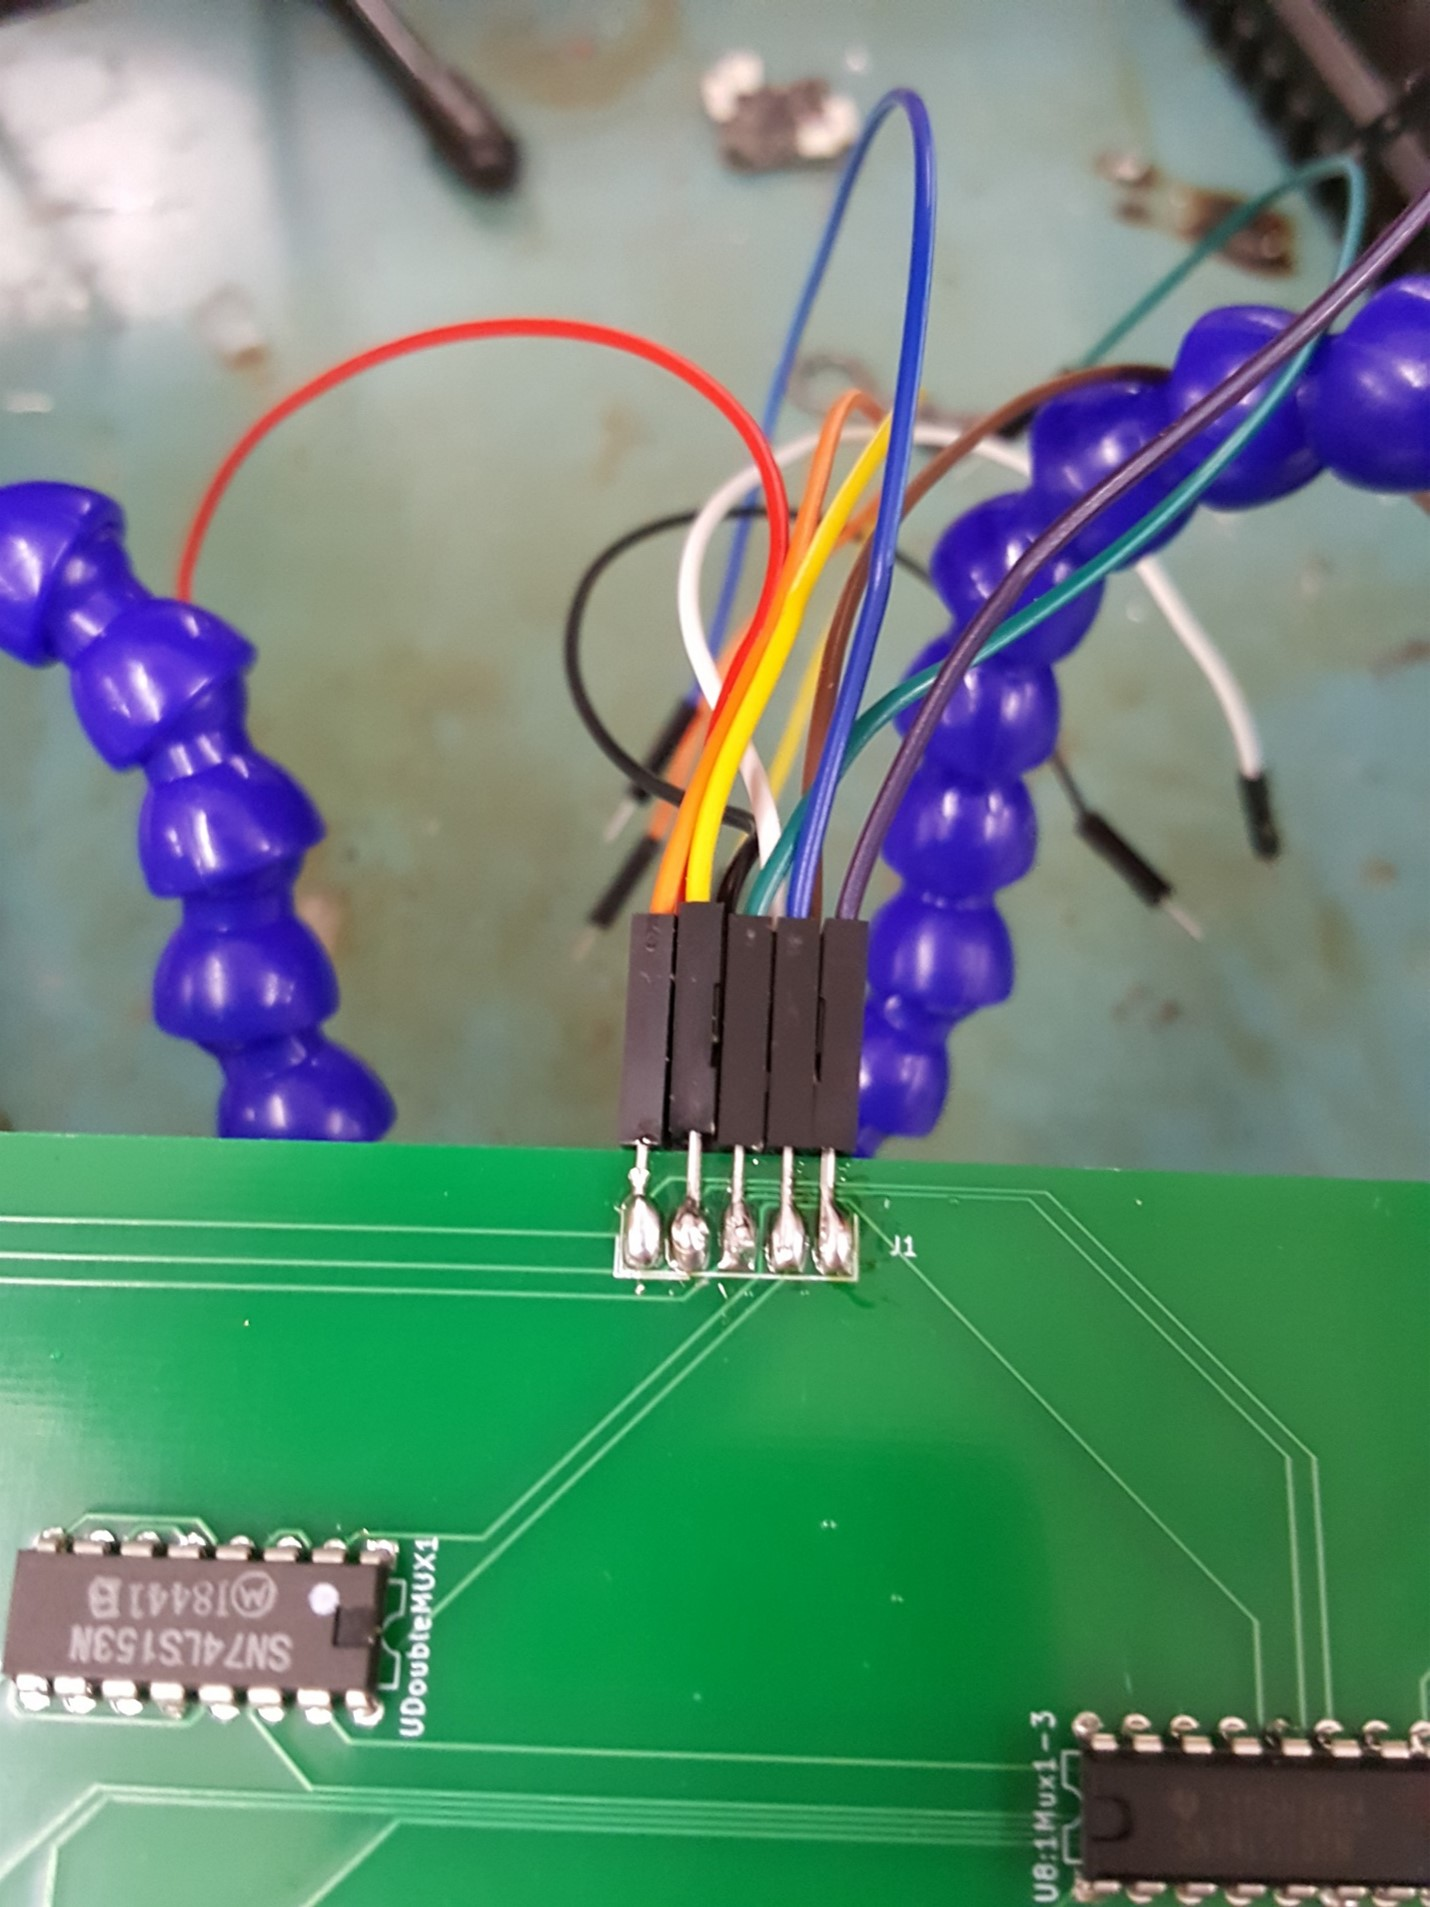
\includegraphics[width=\linewidth]{image/pcbwires.jpg}
  \caption{The wires attached to the PCB.}
\end{figure}

With this completed circuit, it was only a matter of creating a proper and functional
Arduino code to signal and measure the ports on the circuit to determine the velocity of
each subsequent keys. This and the subsequent testing of the given inputs will be
discussed in the following section.
